\documentclass{strrespaper-trad}
\usepackage[utf8]{inputenc}
\usepackage[T1]{fontenc}
\usepackage{csquotes}
\usepackage[english]{babel}

% For math
\usepackage{amsmath}

% For better tables
\usepackage{longtable}
\usepackage{booktabs}
\usepackage{threeparttable}

% For images
\usepackage{graphicx}

% For subfigures
\usepackage{subfig}

% For landscape pages
\usepackage{pdflscape}

% For drawing
\usepackage{tikz}
\usetikzlibrary{shapes.multipart}

% For plotting
\usepackage{xcolor}
\usepackage{pgfplots}
\pgfplotsset{compat=1.16}

% For units
\usepackage{siunitx}
\sisetup{
	separate-uncertainty=true
}

% For Project Plan
\usepackage{pgfgantt}
\usepackage{tabularx}

% For code listings (type "texdoc listings" [without the quotes] for more information)
% \usepackage{listings}

\newcommand{\mnk}{\textit{m, n, k} game}
\newcommand{\mnkpl}{\textit{m, n, k} games}
\newcommand{\ttt}{Tic-Tac-Toe}
\newcommand{\TTT}{TIC-TAC-TOE}

% Required for the citations
\usepackage[style=apa,sortcites=true,sorting=nyt,backend=biber]{biblatex}
\addbibresource{../str-templates/sample-resources/bibliographies/str.bib} % TODO: Remove
\addbibresource{../paleo-str-g12.bib}

 
\title{Comparison of Genetic Algorithm Training Methods As Applied To \ttt}

\usepackage[calc]{datetime2}
\makeatletter
\newcommand{\daymonthyear}{\@dtm@day\ \DTMenglishmonthname{\@dtm@month} \@dtm@year}
\makeatother
\date{\daymonthyear}

\tptitle{
	Comparison Of Genetic Algorithm Training Methods\\
	As Applied To \TTT
}
\addAuthor{Vash Patrick B. Ancheta}
\addAuthor{Diego Sulayman R. Pascua}
\addAuthor{Resh Vnzi S. Togue\~no}
\adviser{Kaye Melina Natividad B. Alamag}
\level{3}

\begin{document}
	\maketitle

	\frontmatter

	\unnumchapter*{APPROVAL SHEET}
		\makeapprovalsheet{
			\signatureline{Conrado C. Rotor, \NoCaseChange{Jr., Ph.D.}}{Chair}

			\signatureline{Melba C. Patacsil}{Co-chair}

			\vspace*{\baselineskip}

			\begin{multicols}{2}
				\begin{center}
					\signatureline{Jay Jay F. Manuel}{Member}
					\signatureline{Ricarido M. Saturay, \NoCaseChange{Jr.}}{Member}

					\columnbreak

					\signatureline{Marites P. Rivera}{Member}
					\signatureline{Freda M. Wong}{Member}
				\end{center}
			\end{multicols}
		}

	\unnumchapter*{ACKNOWLEDGEMENT}
		We are grateful for our friends and family for their continued support in our continuous lives.
		We are also thankful to our teachers, research teacher, and research adviser for their unwavering assistance in having the research completed.
		Without these people, this research would never be successful.

	\unnumchapter{ABSTRACT}
		% TODO: Abstract
		% Do note that abstracts should not contain references.
		\makeabstract{
			According to \textcite{georgemasonuniversityWritingAbstract2020}, \blockquote{An abstract is a 150- to 250-word paragraph that provides readers with a quick overview of your essay or report and its organization. It should express your thesis (or central idea) and your key points; it should also suggest any implications or applications of the research you discuss in the paper.}
			\textcite{georgemasonuniversityWritingAbstract2020} also states that the common abstract is divided into such: 25\% of space on the purpose and importance of the research (Introduction), 25\% of space on what was done (Methods), 35\% of space on what was found (Results), and 15\% of space on the implications of the research.
		}

	\unnumchapter*{Table of Contents}
		\contents
		% \listoflistings

	\mainmatter

	\chapter{INTRODUCTION}
		\section{Background of the Study}
			% TODO: Background of the Study
			Machine learning (ML) is vast---it is used in different situations such as spam detectors, web search engines, photo tagging applications and game development \autocite{sharmaMachineLearningApplications2016}.
			There have been researches that are aimed at improving the implementation of ML in various games.
			A category of games under investigation through ML is the set of \mnk\ games, comprised of games where there is an $m \times n$ grid and two players alternate turns trying to earn $k$ pieces adjacent to each other horizontally, vertically or diagonally \autocite{hayesDevelopingMemoryEfficient2016}.
			Among the most common examples of \mnkpl\ are G\=o, Othello, and Chess.
			\ttt, the game under investigation in this study, is an example of an \mnk.
			A \ttt\ board is composed of three rows and three columns, and requires three adjacent pieces of the same player to render a win, thus it is considered to have a $3, 3, 3$ configuration.

			Improvements in ML have lead to the development of artificial intelligence (AI) players that can beat even the most competitive human players around the world.
			Machine learning methods (MLMs) are algorithms where machines are not explicitly programmed to do what is tasked.
			Rather, similar to its namesake, MLM-trained machines are capable of performing tasks given its own internal code without any human interference.
			In short, the machine \textit{learns} \autocite{geeksforgeeksMachineLearning}.
			An example of an MLM is the genetic algorithm (GA).

			This study aims to develop multiple GAs with different elite preservation methods and compare their performance in \ttt\ based on the possible situations.

		\section{Objectives of the Study}
			\subsection{General Objective}
				\begin{itemize}
					\item To compare the effectiveness of trained genetic algorithm (GA) organisms among each other as applied to \ttt
				\end{itemize}
			\subsection{Specific Objectives}
				\begin{enumerate}
					\item To implement known heuristics into Python code
					\item To train organisms of an implemented GA using different move generators (MGs)
					\item To compare the development of the performance of trained GA organisms among each other within 500 generations
				\end{enumerate}

		\section{Significance of the Study}
			% TODO: Significance of the Study
			This study contributes to the body of knowledge in ML.
			Through this study, more can be known about how information gained from one method of AI can be passed on to another mechanism of AI through training.
			This sheds light on how information from one AI player can be transmitted to an MLM such as GA.
			This, by extension, can improve the comprehension of how machines can learn strategies in games from one with greater skill.

		\section{Scope and Limitations of the Study}
			% TODO: Scope and Limitations of the Study
			This study focuses only on \ttt\ and not other games such as Chess or G\=o because it is the simplest game to conduct the research on heuristics, namely the training of the GA under different MGs.
			The complexity of the board game is not relevant to the study because the focus of the research is to compare the effectiveness of trained GA organisms given an \mnk.
			Applying these heuristics on other \mnkpl\ however are beyond the time frame of the research.
			Only three GAs were developed in this study.
			The first is a Python implementation of the GA in the work of \textcite{bhattSearchNolossStrategies2008}.
			Using developed AI, the second and third are modified implementations of the same GA.
			The performance of each GA is based on how many generations it takes for the GA to find a no-loss first player for \ttt.
			This basis for comparison of performance, specifically using the skill of an organism as a first player, is due to the fact that Python is known for being slow.
			In line with this, indices are 0-based in this paper, as they are in Python.

	\unnumchapter{DEFINITION OF TERMS}
		% TODO: Definition of Terms
		\termdef{\mnk}{
			a game where there is an $m \times n$ grid where two players alternate turns trying to earn $k$ pieces adjacent to each other horizontally, vertically or diagonally
		}
		\termdef{Artificial Intelligence (AI)}{
			program that simulates human actions, can simulate a human player in a game.
		}
		\termdef{Allele}{
			the configuration value of a gene given a unique organism
		}
		\termdef{Genetic Algorithm (GA)}{
			algorithm that simulates natural selection and biological reproduction to produce solutions to a problem
		}
		\termdef{Gene}{
			representation of a unique and distinct situation in a game given the game rules
		}
		\termdef{Genome}{
			mapping table of genes with corresponding alleles
		}
		\termdef{Machine Learning (ML)}{
			a heuristic where a program learns rather than strictly follow a given instruction
		}
		\termdef{Machine Learning (MLM)}{
			algorithms used in machine learning
		}
		\termdef{Organism}{
			an algorithm represented by a genome
		}
		\termdef{Probability Valuation (PV)}{
			classical probability of a player winning at a given game state
		}
		\termdef{\ttt}{
			\mnk\ configured as 3,3,3
		}

	\chapter{REVIEW OF RELATED LITERATURE}
		% TODO: Review of Related Literature
		\section*{Effective Computer Algorithms on \ttt}
			There have already been precedents in investigating the proper method of winning classic \ttt.
			Examples such as prioritizing the center or placement of pieces in the opposite cell of the opponent's previous move are frequently cited as techniques to beat the opponent \autocite{aycockHowWinTicTacToe2002}.
			Multiple discussions gave occurred on how many distinct games one can play in \ttt.
			\textcite{schaeferHowManyGames2002} argues that the common answer of 9! or 362,880 possible games is misleading for it ignores the symmetrical properties of the game.
			There are games that have exactly the same pieces placed on the board but are oriented differently in relation to the board.
			For example, a gametree turned 90\textdegree\ is considered a distinct game state in the 9! calculation.
			According to \textcite{schaeferHowManyGames2002}, it is of more concern to count game states that end when there are $k$ adjacent pieces.
			Using this method of counting game states, \textcite{schaeferHowManyGames2002} computed a total number of 765 distinct game states.

			Numerous studies have been performed on the most effective algorithms for a computer program to win in \ttt.
			In organizing the results of a computer algorithm, one of the most common methods of organization is the use of a game tree.
			A game tree is a collection of all possible game states arranged in chronological order.
			The root node represents the current state, its child node the set possible game states.
			The edges represent the moves and the terminal nodes represent game states that indicate a completed game.
			The game tree begins from the root node and branches out into nodes that have their own children \autocite{adamchikGameTrees2009}.
			A diverse game tree is optimal for exploring the capabilities of the different machine learning methods to be used in the study.

			\begin{figure}
				\centering
				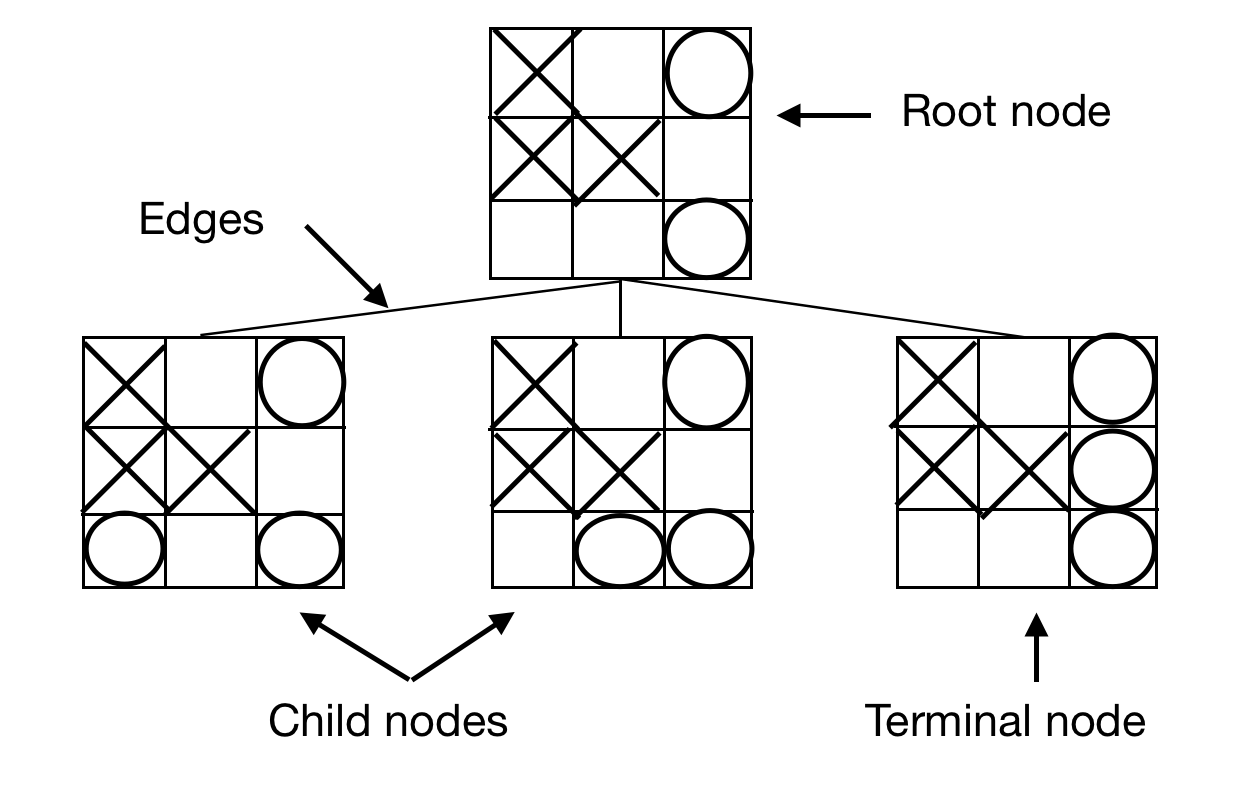
\includegraphics[width=0.7\linewidth]{gametree}
				\caption{Game tree}
				\label{fig:gametree}
			\end{figure}

			A study by \textcite{cranenburghTicTacToe2007} is concerned with the use and implementation of a heuristic known as depth-first search. Depth-first search is a machine learning method that utilizes \textit{backtracking}.
			When the algorithm encounters a terminal node, it returns to the previous nodes to find other possible nodes, hence the term \textit{backtracking} \autocite{hackerearthDepthFirstSearch2019}.
			According to \textcite{cranenburghTicTacToe2007}, a higher depth search with more game states, leads to a higher win rate or at least, leads the program to reach a draw better.

			Researches that deal with the more complex \ttt\ variant Ultimate/Super \ttt\ seek to find the patterns and implementing these patterns into AI.
			Analogous to how classic \ttt\ is symmetric, a study by \textcite{georgeGroupActionsWinning2016} specifies the rotational and reflectional symmetry of Ultimate/Super \ttt.
			A study by \textcite{lifshitzAIApproachesUltimate} deals with the use of a mixture of heuristics and algorithms such as MiniMax (an algorithm that traverses the whole game tree) and ExpectiMax (an algorithm that analyzes the expectations of the opponent's moves).
			Given a controlled set of parameters, ExpectiMax won against a random algorithm most of the time.
			When played against MiniMax however, ExpectiMax was more likely to lose.
			This is in agreement with the aforementioned conclusion that an increased depth produces better results.
			A caveat for this machine learning method is the drastic duration of time the algorithm requires with each increase in depth.
			The higher the depth of the depth-first search, the longer the time needed for the algorithm to provide the most optimal move.

		\section*{Machine Learning Methods}
			Various methods of machine learning have been discovered prior.
			One of the earliest examples of machine learning methods is Hexapawn formulated by Martin Gardner.
			The game is composed of a $3 \times 3$ board with two sets of three pawns in a row on opposite sides of the board, and the players move alternately.
			The game is typically played by a human (who always goes first) and an AI player.
			A player wins the game by accomplishing one of three goals: move a pawn to the opposite edge, capture all enemy pieces, or leave the enemy with no moves.
			Because of the small scale of the game and its symmetry, all the possible game states can be represented in 24 cards.
			Each of these cards contains a move performed by the human player and arrows of different colors representing the possible moves the AI player can take \autocite{ortizMachineLearningHexapawn2017}.
			The AI player contains a matchbox for each card representing a game state.
			These matchboxes contain beads that correspond to the possible moves the AI player may make.
			During play, the beads are chosen at random and the AI player moves according to the bead taken.
			If the move made by the AI player leads to the loss of the AI, the bead corresponding to the move is taken away.
			Otherwise, the bead is returned to the matchbox.
			After 50 games, the AI player is practically unbeatable as game states with high probability of loss is reduced \autocite{gardnerMathematicalGames1958}.

		\section*{Genetic Algorithm}
			Living organisms exhibit a level of problems solving that is almost impossible to be recreated by a computer scientist.
			Even more, the complexity that living organisms show is one that is incredibly enviable to a computer scientist wanting to achieve some problem solving program; problems that computer scientists have spent endless amounts of intellectual effort on have been solved by living organism without any thought, relying on the process of evolution.

			Due to this, many researchers have began emulating the process of evolution on their algorithms, subjecting their own programs to a process of reproduction and natural selection.
			This method is widely used in the realm of machine learning, since it eliminates a great hurdle in software engineering: programmers need not to specify the individual aspects of each program and the means that actions are carried out.

			\begin{figure}
				\centering
				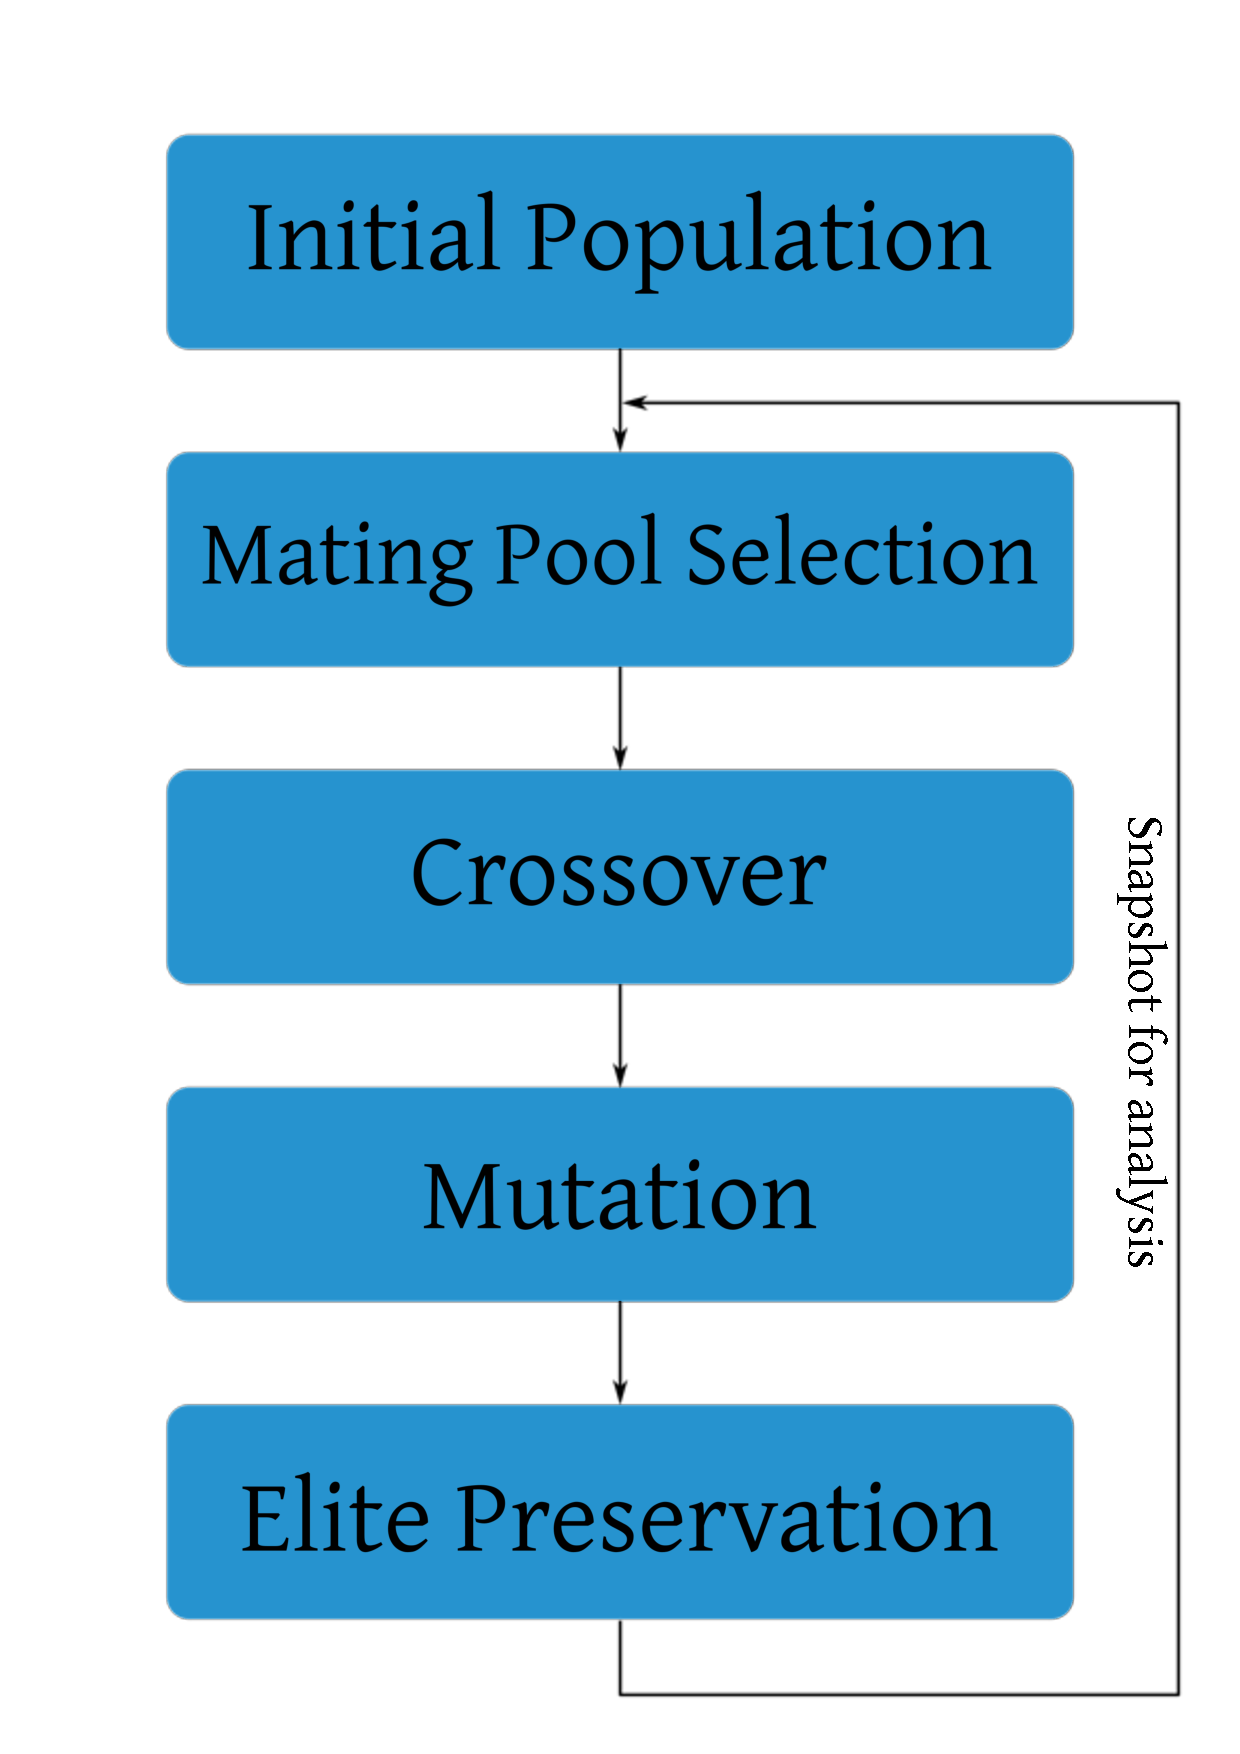
\includegraphics[width=0.6\linewidth]{genetic}
				\caption{Flowchart of GA training}
				\label{fig:genetic}
			\end{figure}

			There are two aspects of the evolution process that computer scientists want to emulate: natural selection and reproduction. "Natural selection" is the process of choosing which solutions survive to make a new generation of algorithms, the survivors govern the characteristics of next generation. Reproduction is the recombination of genes from parent to offspring, making the "child" algorithm of an organism have similar characteristics to their two parent algorithms.

			Programming natural selection is done by giving an algorithm a test of fitness, going through numerous iterations, then giving a fitness score based on that performance \autocite{hochmuthGeneticEvolutionPerfect2003}.
			Fitness scores are usually calculated based on the ratio of games won, as shown in Equation~\ref{eqn:fitness}.
			The higher the fitness score, the higher the changes of winning with the solution or the move done in the game.
			Algorithms with low fitness scores are discarded and those with high fitness scores move on to reproduction.
			\begin{equation}
				f(x_i) = \frac{n_\mathrm{lost}}{n_\mathrm{games}} \label{eqn:fitness}
			\end{equation}
			The emulation of reproduction is far more complicated.
			Originally, it was based on random mutation of the algorithms, however this oftentimes produces algorithms that would not run, or are drastically different from the intended purpose of the program.
			Later development focuses on adding together characteristics from the two parents.
			This was also limited since this could only be done to characteristics that could be added meaningfully \autocite{hollandGeneticAlgorithms}.

			Currently, reproduction is done by means of a classifier system.
			A classifier system is a system where conditions and actions are represented by strings of ones and zeroes corresponding to the presence or absence of that characteristic.
			For example, as shown in Table \ref{tab:ex_classifier}, since humans have eyes and opposable thumbs and require oxygen, but do not have wings or gills, humans can be recorded as [10011], while the only recorded characteristic of the bacterium that is present is that it requires oxygen, so it is recorded as [00001].
			Reproduction can now be done on these "genes" by recombining different genes and making new offspring.
			In the computer science world, these aspects are usually very basic and primitive, but with strings with lengths reaching tens of thousands of bits long.

			\begin{table}[htbp]
				\centering
				\begin{tabular}{lccc}
					\toprule
					Aspect           & Human & Fish & Bacterium \\
					\midrule
					opposable thumbs & 1     & 0    & 0         \\
					wings            & 0     & 0    & 0         \\
					gills            & 0     & 1    & 0         \\
					eyes             & 1     & 1    & 0         \\
					requires oxygen  & 1     & 1    & 1         \\
					\bottomrule
				\end{tabular}
				\caption{Example of Organisms Sorted Through a Classifier System}
				\label{tab:ex_classifier}
			\end{table}

	\chapter{MATERIALS AND METHODS}
		\section{Research Design}
			This Developmental Research is composed of two components: Software Development and Data Collection.
			In Software Development the code for the move generators and genetic algorithms are initialized, and the efficiency of its implementation is optimized.
			In Data Collection the organisms were trained for 500 generations, and the fitness data collected was analyzed using $R$.
			The independent variable is the elite preservation method.
			The dependent variable is the number of generations the specific GA takes to find a no-loss solution.
			Extraneous variables such as the software specifications can be held constant by the use of the same software such as the operating system and the same Python version (3.8.3 64-bit).
			The study was not affected by hardware specifications as it concerns the number of generations instead of the time taken on the system.

		\section{Locale of the Study}
			The software was developed and data was collected mainly at the Philippine Science High School -- Cordillera Administrative Region Campus.
			The training and data collection occurred at the aforementioned location on various personal computers.

		\section{Materials and Research Instruments}
			The software was developed with Python 3.8.3 on KDE Neon 5.18 using Visual Studio Code 1.45.1 and hosted on GitHub.
			A link to the repository hosting the software is located in \ref{apx:documentation}.
			The developmental computer is equipped with 4 GB of Random Access Memory (RAM).
			Various personal computers were used to perform the training.

		\section{Procedures}
			\subsection{Software Development}
				The study aims to compare the performance of the genetic algorithms with different elite preservation methods.
				The three are: an unmodified Python implementation of the work of \textcite{bhattSearchNolossStrategies2008}, and two with modified elite preservation methods based on MGs.
				A preliminary for the accomplishment of such task is a game engine for the interaction between trained GA organisms.
				This was coded in Python, as application programming interfaces (APIs) for machine learning have already been implemented in Python.

				After the development of a platform for play of \ttt\ between trained organisms, the development of the required MGs followed.
				The Random Move Generator (RMG) returns one of all possible moves in \ttt\ with equal probability.
				Another MG is Unbeatable Move Generator (UMG).

				UMG is based off of the work of \textcite{barratRobbiebarratUnbeatableTictactoe2019}.
				It is stated to be unbeatable, however, due to the fact that there are random moves involved in the code, the Move Generator has a small chance of being beat.
				This makes an ideal opponent for trained organisms, given that the GA will find an exploit eventually.
				In line with this, the GA might be able to use said exploit to have better performance.

				\paragraph{Genetic Algorithm}
					The organisms to be trained were implemented in Python as well.
					The GA was composed of unique genomes with genes for each possible game state with alleles that correspond to the moves to be taken.
					Following the flow represented in Figure~\ref{fig:genetic}, the operators are adapted from \textcite{bhattSearchNolossStrategies2008}.
					The only aspect of the GA that differs from the implementation of that in \textcite{bhattSearchNolossStrategies2008} is the organism representation.
					\subparagraph{Organism Representation}
						Organisms are represented with genomes, as shown in Figure~\ref{fig:genome}.
						Each gene in the genome represents a game state that considers rotation and symmetry using an implementation of the game-base used by \textcite{bhattSearchNolossStrategies2008}.
						These genes have a corresponding allele that represents the move the organism will take.
						\begin{figure}[htbp]
							\centering
							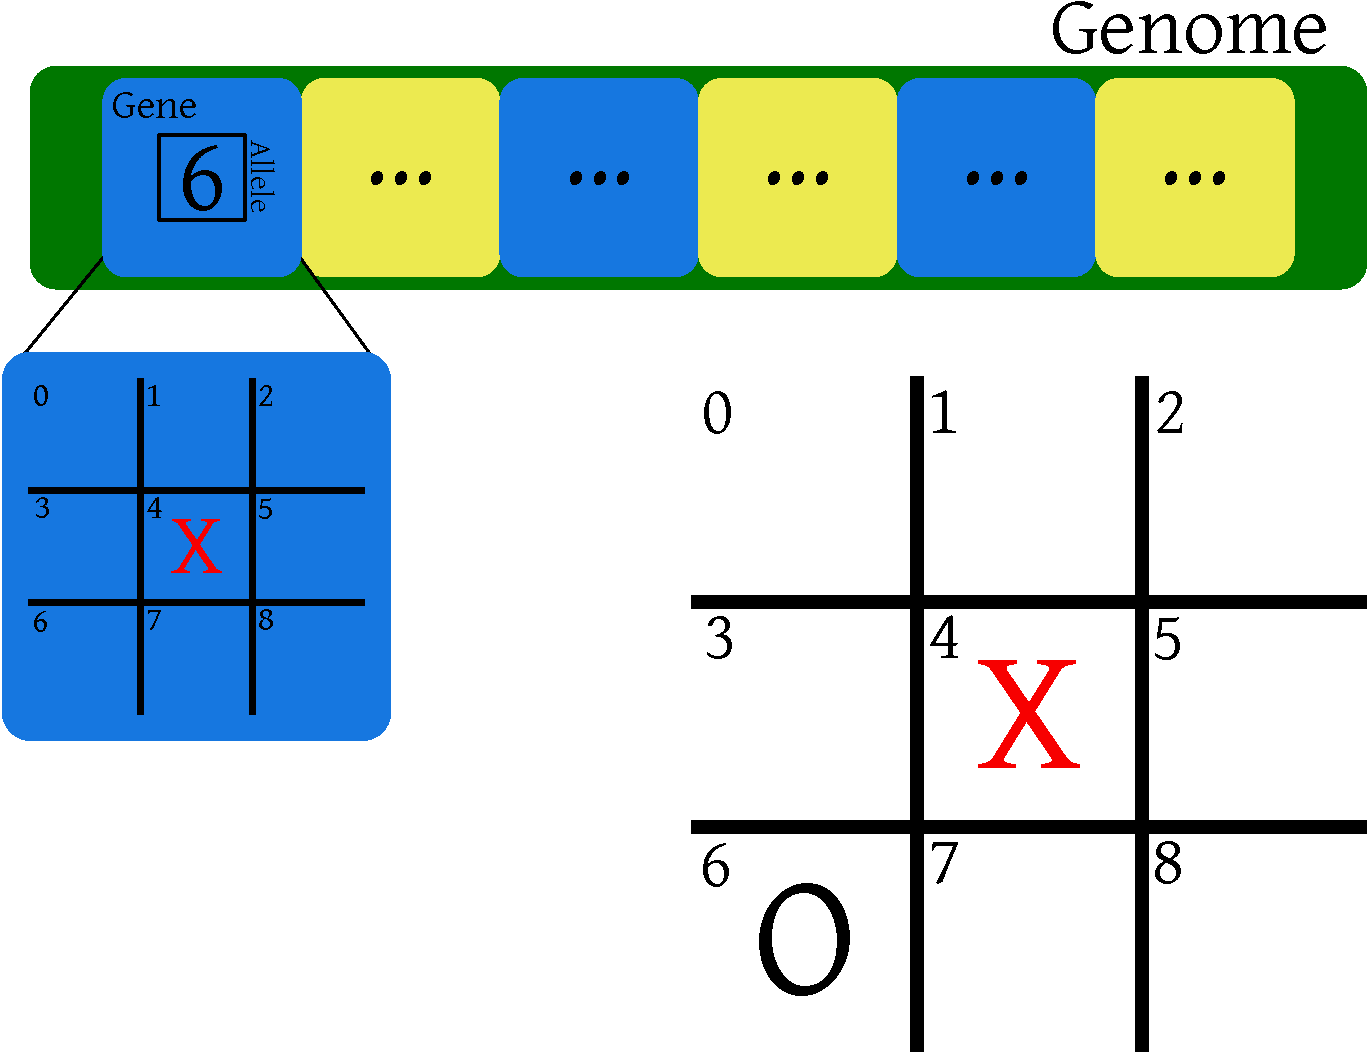
\includegraphics[width=0.75\textwidth]{representation}
							\caption{Genome of an organism}
							\label{fig:genome}
						\end{figure}
					\subparagraph{Initial Population}
						For each game state represented by genes in the genome, the organism is given a random possible move for that game state.
						Any valid move in a given game state is considered in choosing the allele randomly.
					\subparagraph{Selection Operator}
						Using a modified implementation of the Stochastic Universal Selection (SUS) Operator by \textcite{panchapakesanStochasticUniversalSampling2014}, the following niched fitness equation was used \autocite{bhattSearchNolossStrategies2008}:
						\begin{equation*}
							f_\mathrm{niched}(x_i) = \frac{1}{m} * [1 - f(x_i)]
						\end{equation*}
						where $m$ is the number of organisms with the same fitness.
						In this specific case, half of the population is selected via SUS.
					\subparagraph{Crossover Operator}
						Similar to that of \textcite{bhattSearchNolossStrategies2008}, 50 cross-sites are randomly chosen per parent pair which is used to take alternate series of alleles from each parent.
						This produces two new offspring with alleles from each parent.
						The mating pool is linear, with parent pairs formed from a mating pool individual and the individual adjacent to it.
						If the individual is last in the linear mating pool, it is paired with the first individual in the mating pool.
					\subparagraph{Mutation Operator}
						Using random reset mutation, $n_m$ genes are mutated based on the best fitness in the population.
						This basis is formalized by \textcite{bhattSearchNolossStrategies2008} in the following equation:
						\begin{equation*}
							n_m = 250 * f_\mathrm{minimum} + 10
						\end{equation*}
					\subparagraph{Controlled Elite Preservation}
						In the control genetic algorithm, the organisms from the population before crossover, the population before mutation, and the population after mutation are sorted by fitness in increasing order.
						The solutions with sorted index $j - 1$ are chosen:
						\begin{equation*}
							j(i) = i + 2N * \frac{(i - 1)(i - 2)}{(N - 1)(N - 2)},~~i = 1, 2, \dots, N
						\end{equation*}
					\subparagraph{Modified Controlled Elite Preservation}
						The following modifications were made to the elite preservation method to produce two other GAs:
						In UMG-Controlled Elite Preservation, the organisms are sorted by the number of losses of each organism when played against the UMG for 300 games.
						In RMG-Controlled Elite Preservation, the organisms are sorted by the number of losses of each organism when played against the RMG for 300 games.

			\subsection{Data Collection}
				In the beginning of the GA the organisms were behaving randomly.
				The fitness function for the organisms was based on the possible results based on an unpredictable opponent, thus every possible win, loss and draw is computed and plugged into Equation~\ref{eqn:fitness} to retrieve the fitness of an organism.
				Through natural selection the \enquote{best} organism prevails.
				When the \enquote{best} organism has zero fitness, the GA stops and snapshots the population for the last time.
				If no zero-fitness organism is found before 500 generations have passed, the GA stops itself.
				Using this method, 30 simulations per elite preservation method was run, with 100 organisms per population.
				The number of generations before a simulation encounters a zero-fitness or no-loss solution is recorded for each simulation.

		\section{Treatment of Data}
			\subsection{Statement of Hypotheses} \vspace{-2em}
				\begin{align*}
					H_0 & : \mu_\mathrm{UMG} = \mu_\mathrm{fitness} = \mu_\mathrm{RMG} \\
					H_a & : \text{The means are not all equal}
				\end{align*}
			\subsection{Analysis of Data}
				The data was analyzed through the $R$ with the use of Analysis of Variance (ANOVA) which gives the $p$-value to test the hypotheses at a given confidence interval.
				The study utilizes $\alpha = 0.10$.
				Should the alternative hypothesis be true, Tukey Honest Significant Differences (Tukey HSD) is applied to locate the different mean.

	\chapter{RESULTS AND DISCUSSION}
		\begin{figure}[htbp]
			\centering
			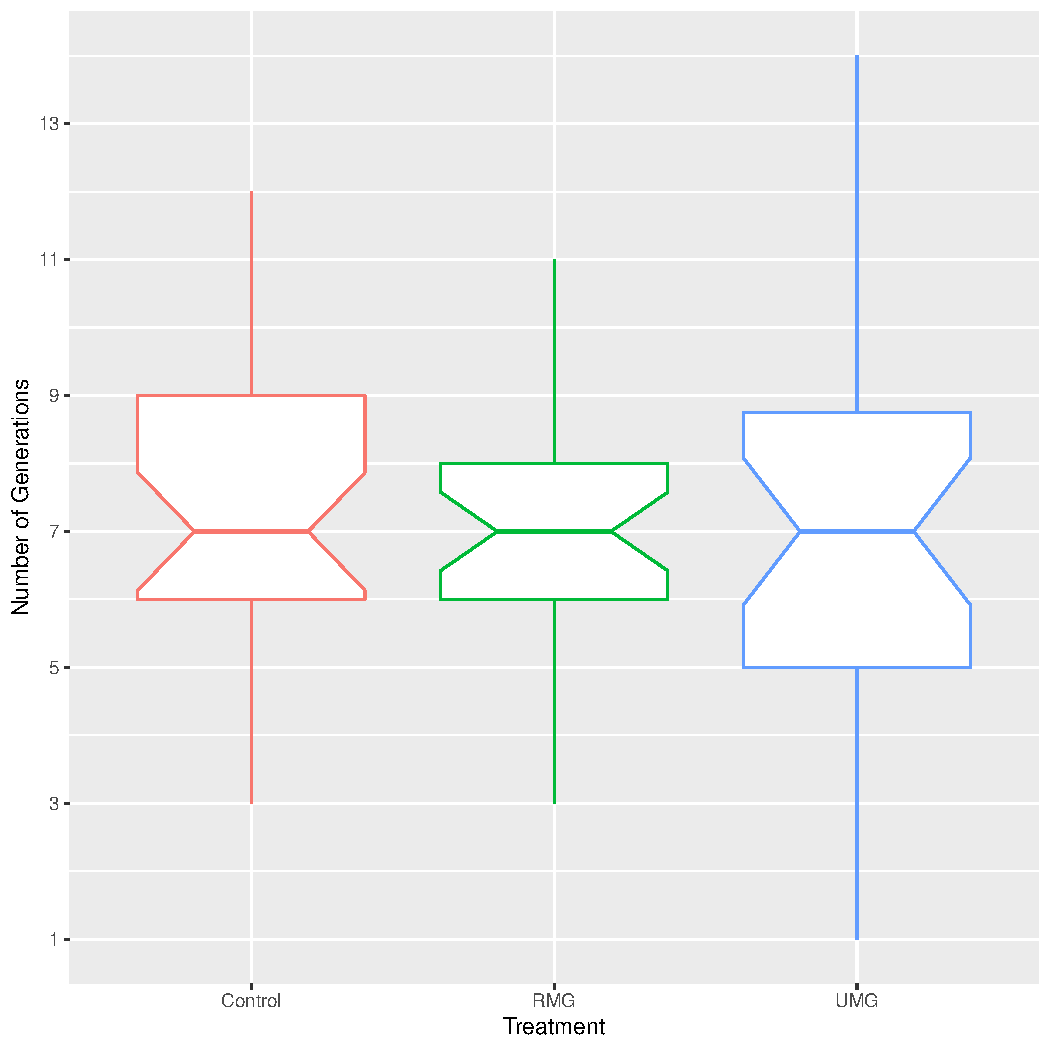
\includegraphics[width=\textwidth]{../figures/boxplot}
			\caption{Notched box plot of treatments}
			\label{fig:boxplot}
		\end{figure}

		A notched box plot of treatment results is shown in Figure~\ref{fig:boxplot}.
		This box plot denotes the interquartile range (IQR) where 50\% of the data is located.
		It is shown that each treatment has a median of seven (7) generations before termination, and the population median is shown by the notches to be within six to eight generations.
		The UMG-controlled GA shows a larger spread while the RMG-controlled GA shows more consistent data points.

		\begin{figure}[htbp]
			\centering
			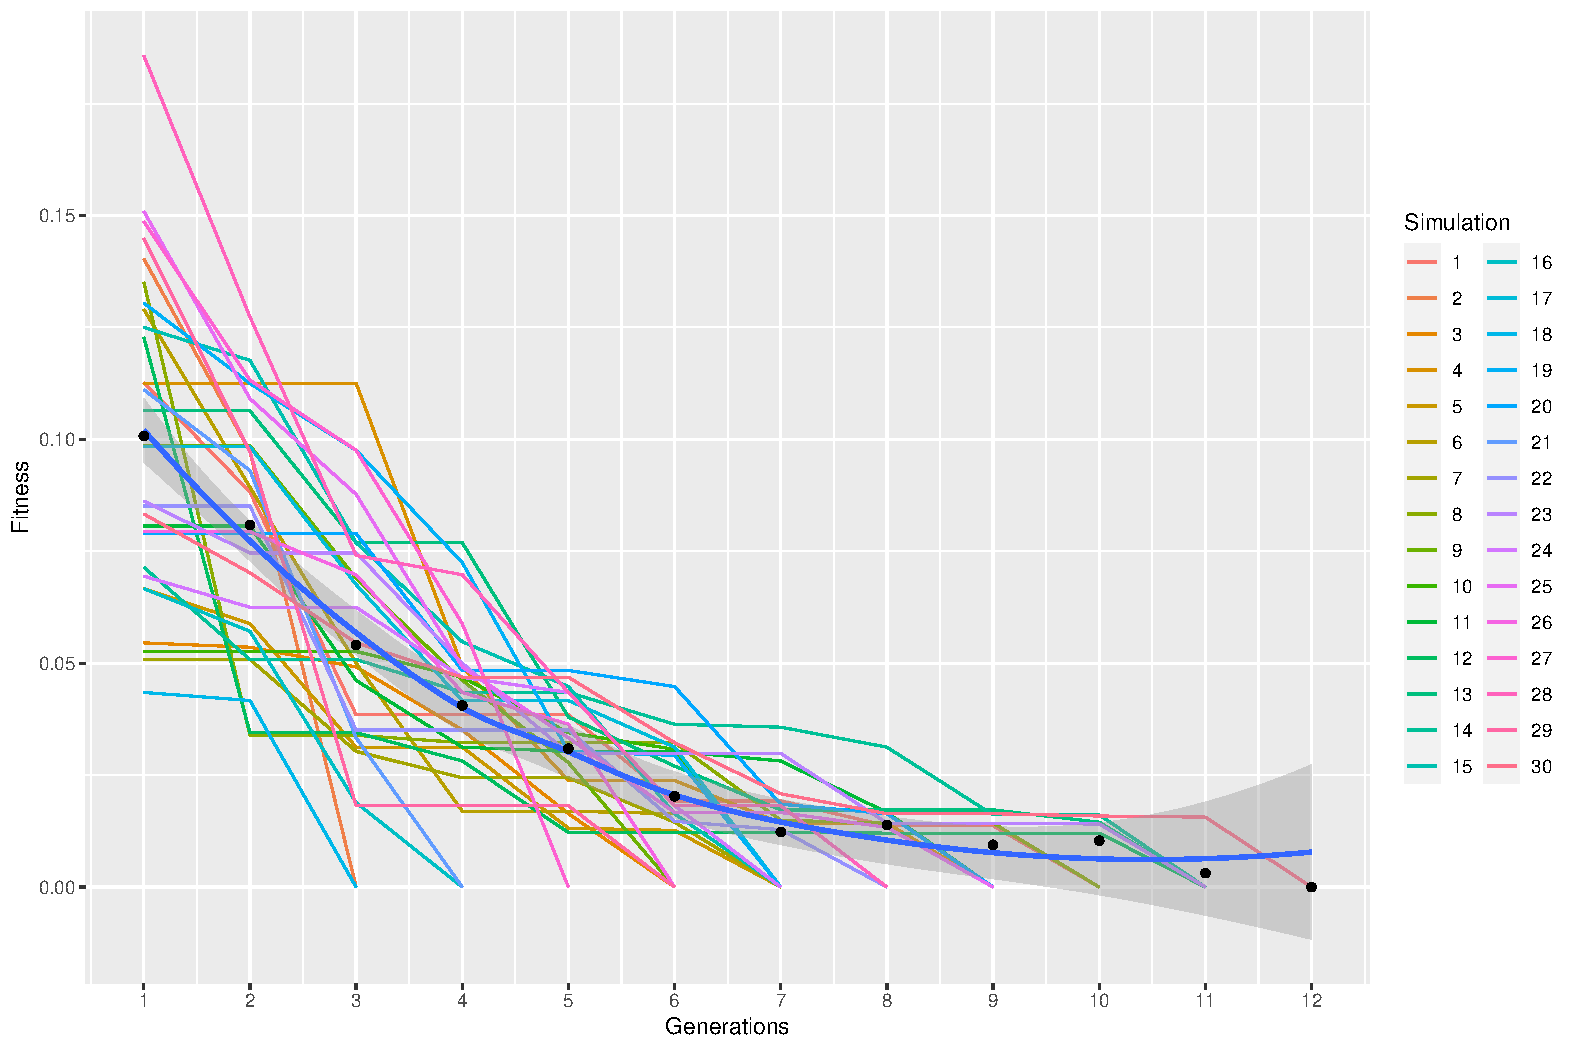
\includegraphics[width=\textwidth]{../figures/ctrl_ftrack}
			\caption{Population-best fitness graph of control}
			\label{fig:fitgraph_ctrl}
		\end{figure}

		The large spread in the data points of the UMG-controlled GA is also evident in Figure~\ref{fig:fitgraph_umg}.
		It is easily shown by the wide standard error bar depicted along the smoothed regression model compared to the standard error bars depicted in Figure~\ref{fig:fitgraph_ctrl} and Figure~\ref{fig:fitgraph_rmg}.
		Figure~\ref{fig:fitgraph_umg} also depicts unique cases where population-best fitness suddenly increases by a large margin.

		This evident spread might invalidate the ANOVA test, thus Bartlett's Test for Homogeneity of Variances was applied to the data via $R$ \autocite{nist/sematechBartlettTest2013}.
		This test resulted in $\chi^2 = 5.1019,~df = 2$ with a $p$-value of 0.07801.
		Said $p$-value is greater than $\alpha = 0.05$, thus the assumption of homogeneity of variances that is necessary in ANOVA is maintained.

		ANOVA was then used to test the null hypothesis that the means of the treatments are equal.
		This returned an F-value of 0.264 and a $p$-value of 0.768.
		The $p$-value is greater than $\alpha = 0.05$, therefore the null hypothesis that the means of the treatments are equal is not rejected.

		\begin{figure}[htbp]
			\centering
			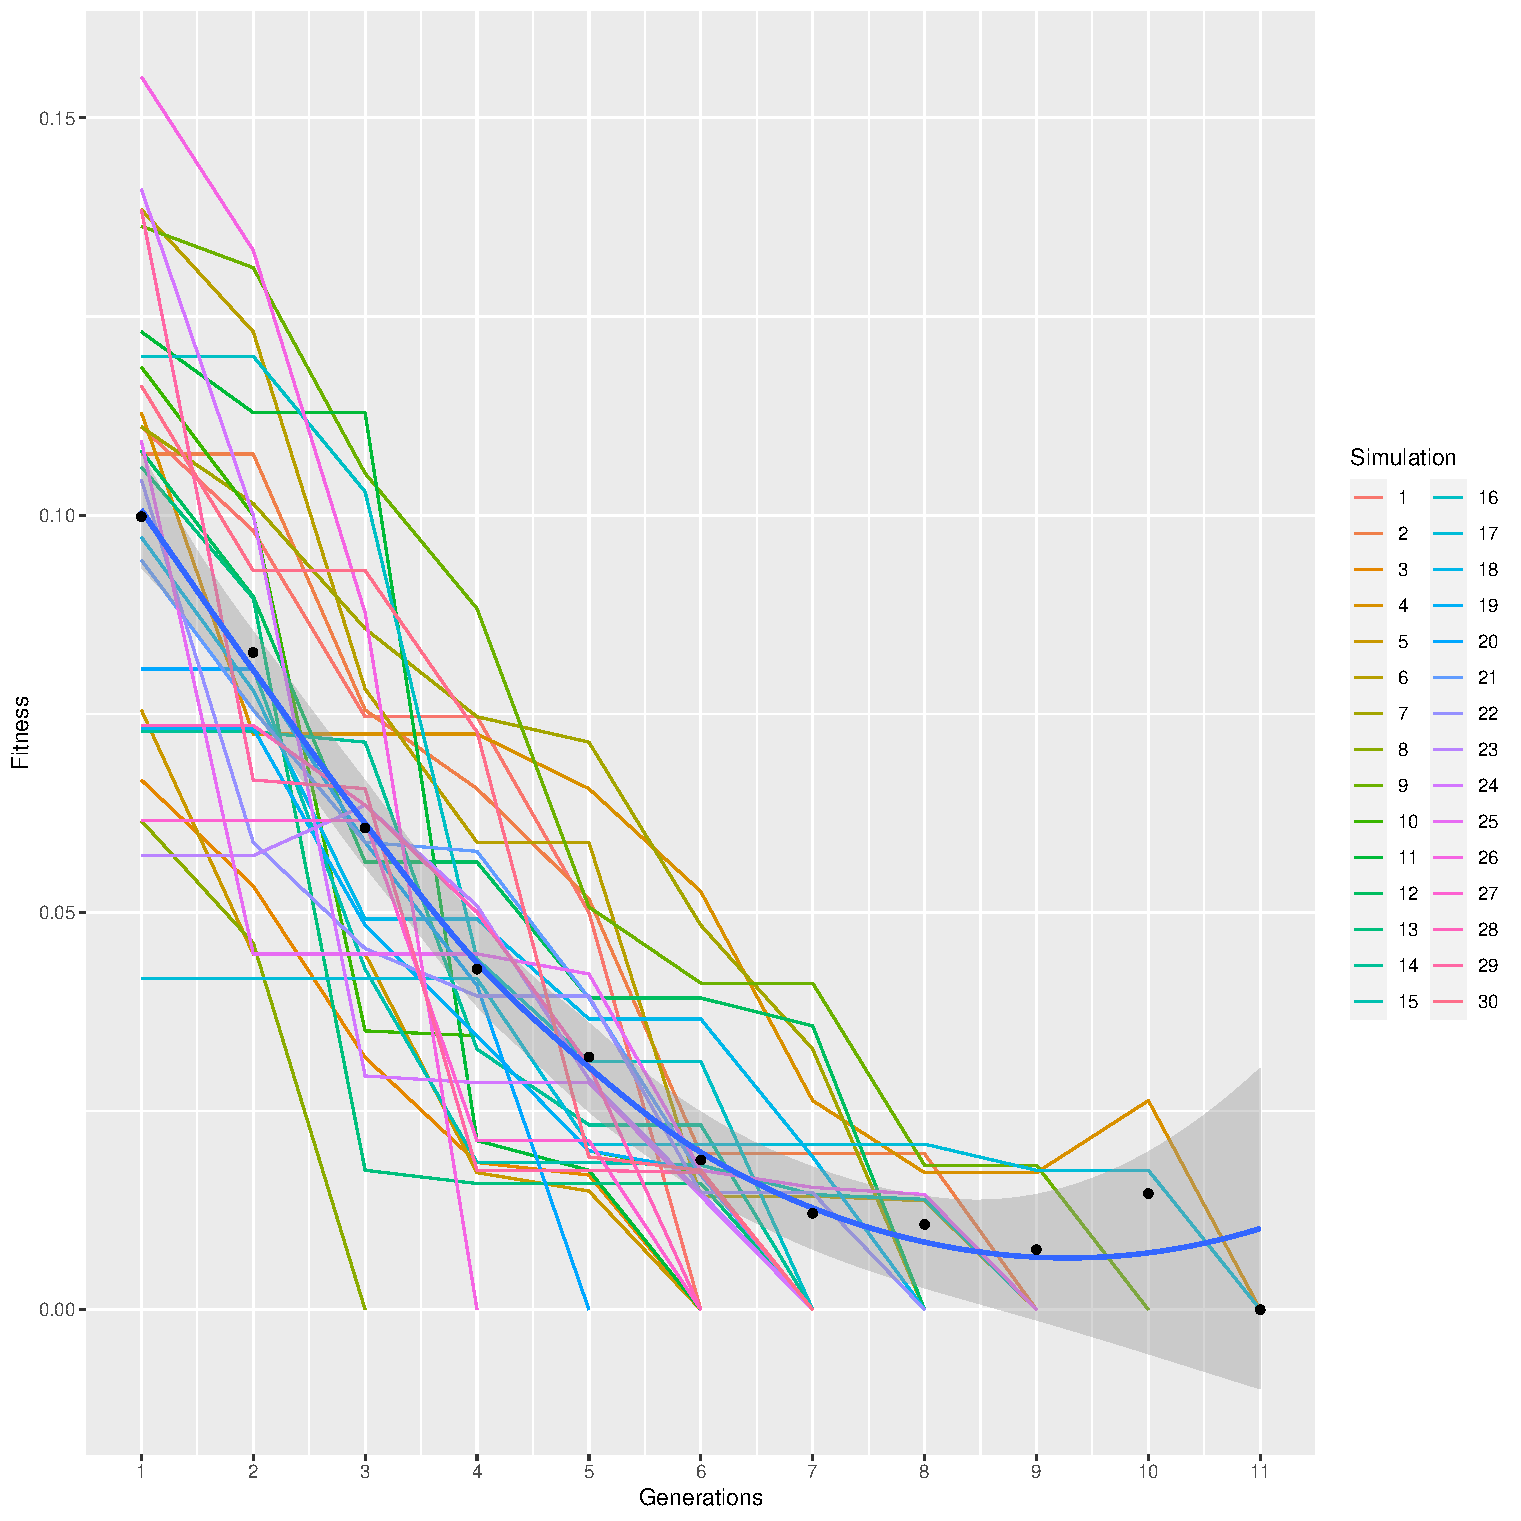
\includegraphics[width=\textwidth]{../figures/rmg_ftrack}
			\caption{Population-best fitness graph of RMG-treated}
			\label{fig:fitgraph_rmg}
		\end{figure}
		\begin{figure}[htbp]
			\centering
			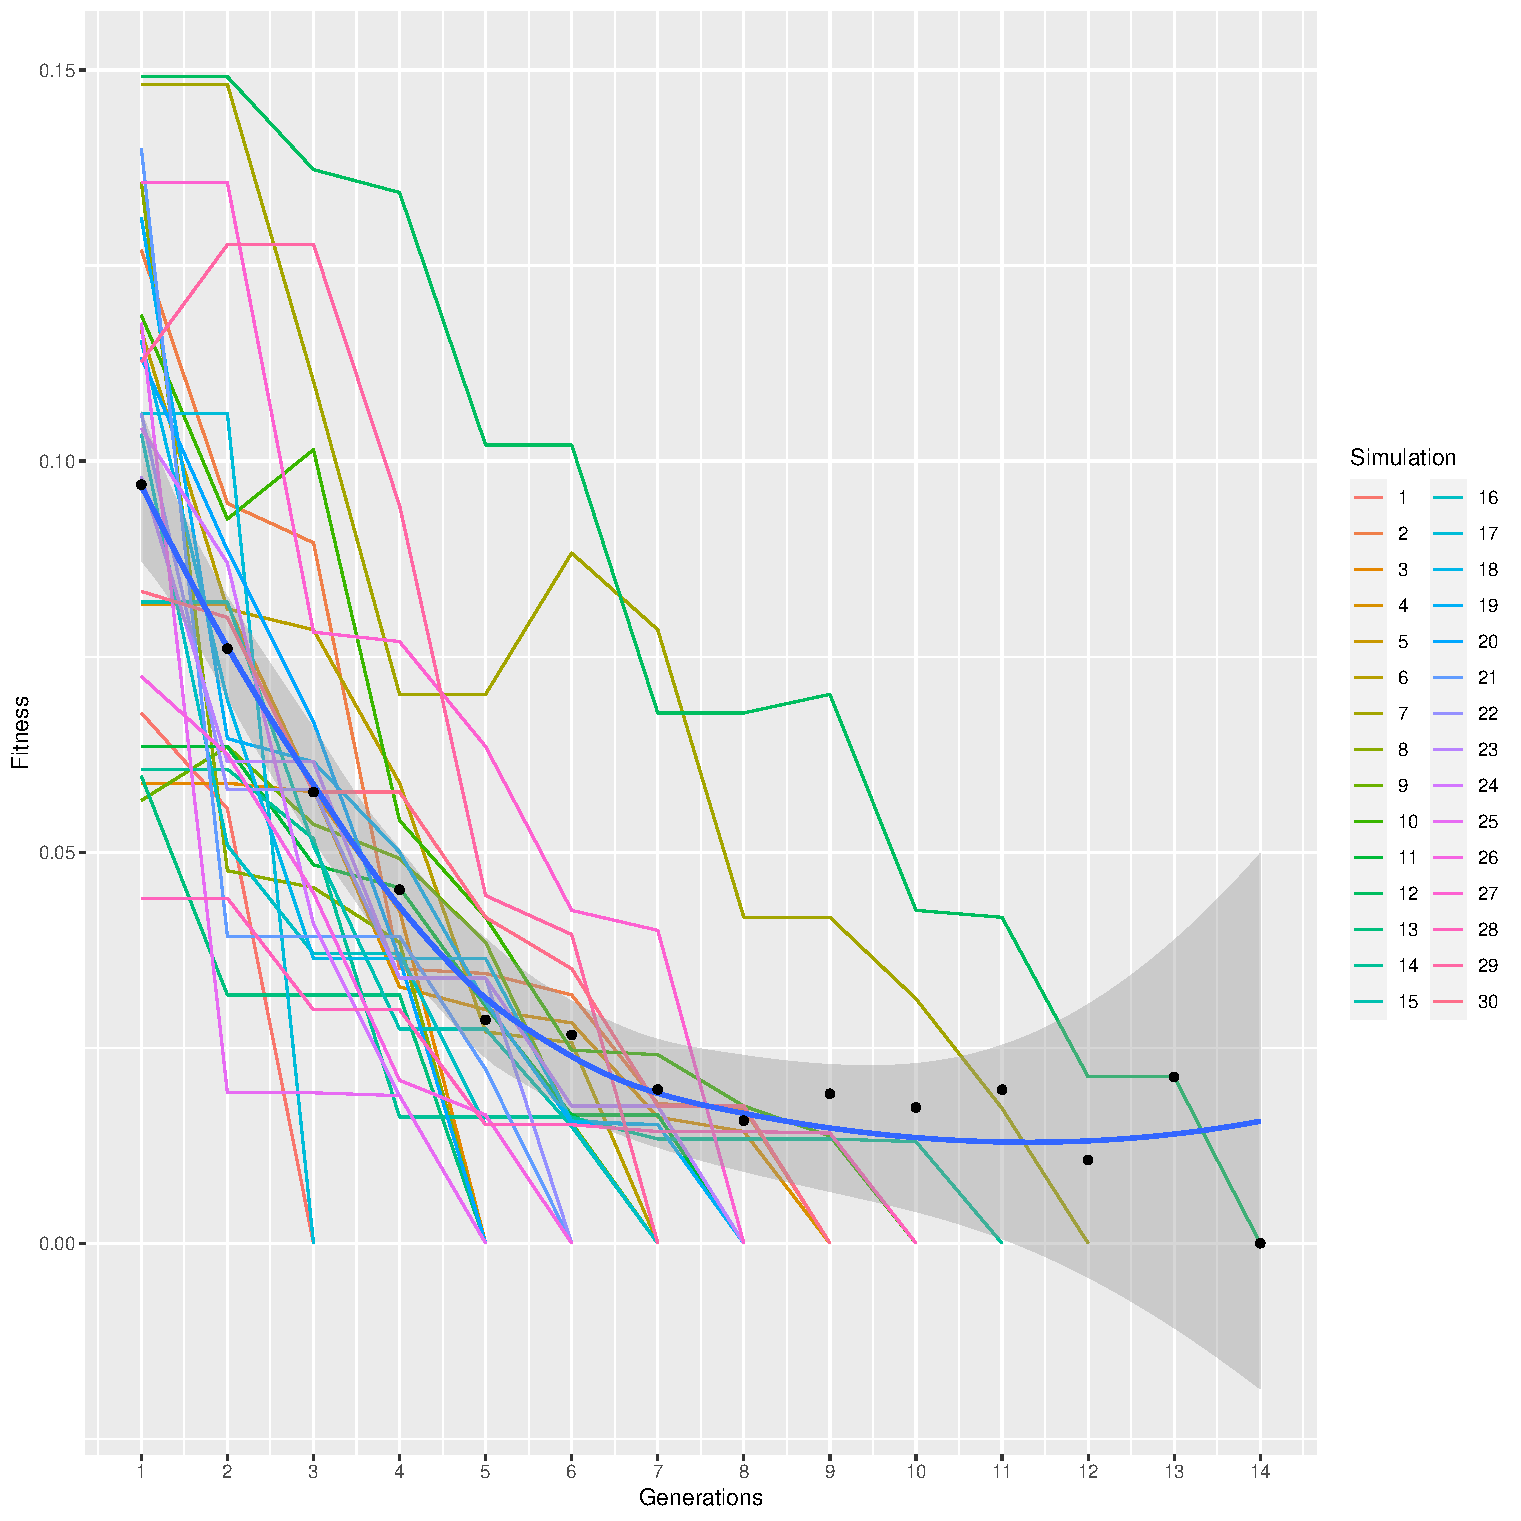
\includegraphics[width=\textwidth]{../figures/umg_ftrack}
			\caption{Population-best fitness graph of UMG-treated}
			\label{fig:fitgraph_umg}
		\end{figure}

		The ANOVA test results assert that the modifications have no effect on the number of generations a GA requires to find a no-loss solution.
		This means that the application of an unbeatable opponent did not promote the genetic evolution of the GA towards a no-loss solution.
		This can imply that either the modification was made in a less-effective component, or the application did not change any behaviour of the GA at all.
		The latter implication can be disproven by the discrepancies produced by the UMG-controlled GA demonstrated in Figure~\ref{fig:fitgraph_umg}.
		This behaviour shows that in some cases, the alignments of the UMG goes against the alignments of the fitness function.
		Such behaviour demonstrates that the UMG modification does in fact, affect the evolution of the GA in no small way.

		In the case that the UMG modification was placed in a less-effective component of the GA, it could be implied that there is no effective component in the GA that can accommodate the modification, or that there is one that is not specifically in the Controlled Elite Preservation operator.
		To prove whether there is an effective component in the GA that can utilize the \enquote{unbeatability} of the UMG or not requires extensive research far beyond the scope of this study.

		Either way, this study shows that modifying the Controlled Elite Preservation operator of the GA does not significantly improve the performance of the GA.
		An observation that might be of use, however, is the fact that the UMG-controlled GA shows promise of increase in variability of the GA, which can be used in finding more diverse solutions in the search space.

	\chapter{CONCLUSION AND RECOMMENDATIONS}
		In essence, the stated objectives: to train organisms with MGs and to compare their performance, has been achieved through the modifications to the Controlled Elite Preservation operator.
		This study targeted the Controlled Elite Preservation operator specifically, thus further research is required to acquire more comprehensive data regarding the effects of having a \enquote{smart} opponent control the evolution of a GA.
		
		The study resulted in proof that modifying the Controlled Elite Preservation operator does not improve the performance of the GA.
		This opens up more questions, on whether or not the application of MG will ever affect the behaviour of a GA.
		It is also recommended to involve testing the performance of the GA as a second player.
		Furthermore, this research serves as a foundation for more extensive investigations into the effects of \enquote{smart} AI on the learning of other AI.

	\literaturecited

	\appendix

	\chapter{Project Plan}
		\begin{table}[htbp]
			\centering
			\caption{Task Lists and Duration}
			\label{tab:task_lists_duration}
			\begin{tabularx}{\linewidth}{cXcc}
				\toprule
				Task & Task Description                                                    & Preceding Tasks & Duration (in days) \\
				\midrule
				A    & Development of \ttt\ Game Platform and Implementation of Algorithms & ---             & 30                 \\
				B    & Testing, Refinement and Optimization of Implemented Programs        & A               & 31                 \\
				C    & Data Collection                                                     & B               & 60                 \\
				D    & Data Analysis                                                       & C               & 60                 \\
				\bottomrule
			\end{tabularx}
		\end{table}

		\begin{figure}[htbp]
			\centering
			\newcommand{\netchart}[8]{
				\node
				[rectangle split,
					rectangle split parts = 3,
					draw,
					minimum width = 3cm,
					font = \small,
					rectangle split part align = {center}
				] (#8)
				{
					\centering
					\begin{tabularx}{2.75cm}{@{} >{\centering\arraybackslash}X|>{\centering\arraybackslash}X|>{\centering\arraybackslash}X @{}}
						#1 & #2 & #3 \\
					\end{tabularx}
					\nodepart{two}
					#4
					\nodepart{three}
					\begin{tabularx}{2.75cm}{@{} >{\centering\arraybackslash}X|>{\centering\arraybackslash}X|>{\centering\arraybackslash}X @{}}
						#5 & #6 & #7 \\
					\end{tabularx}
				};
			}
			\newcommand{\nchconnect}[2]{\draw[->] (#1.two east) to [out=0, in=180] (#2.two west);}
			\tikzset{
				block/.style={
						rectangle,
						draw,
						minimum height=4em,
						minimum width=4em,
						text depth=1em,
						outer sep=0pt,
						font=\small
					}
			}
			\begin{tikzpicture}
				\netchart{0}{30}{30} {Task A} {0}{30}{30} {tA}
				\begin{scope}[xshift=4cm]
					\begin{scope}[yshift=0cm]
						\netchart{30}{31}{61} {Task B} {30}{31}{61} {tB}
						\begin{scope}[xshift=4cm]
							\netchart{61}{60}{121} {Task C} {61}{60}{121} {tC}
						\end{scope}
					\end{scope}
					\begin{scope}[xshift=8cm]
						\netchart{121}{60}{181} {Task D} {121}{60}{181} {tD}
					\end{scope}
				\end{scope}
				\nchconnect{tA}{tB}
				\nchconnect{tB}{tC}
				\nchconnect{tC}{tD}
			\end{tikzpicture}
			\caption{Network chart}
			\label{fig:network_chart}
		\end{figure}


		\begin{landscape}
			\newpage
			\newcommand{\allpersonnel}{
				\begin{tabular}{c}All\\Personnel\end{tabular}
			}
			\newcommand{\threerowdate}[3]{
				\begin{tabular}{c}#1\\#2\\#3\end{tabular}
			}
			\newcommand{\tworowcell}[2]{\begin{tabular}{c}#1\\#2\end{tabular}}

			\begin{table}[ht]
				\centering
				\caption{Task Schedule Management and Personnel Assignment Plan}
				\label{tab:task_schedule_personnel_assignment}
				\begin{tabular}{cccccccc}
					\toprule
					Task & Task Description                                                                   & Personnel     & Duration (in days) & EST                          & LST                          & ECT                          & LCT                          \\
					\midrule
					A    & \tworowcell{Development of \ttt\ Game Platform and} {Implementation of Algorithms} & \allpersonnel & 30                 & \threerowdate{NOV}{01}{2019} & \threerowdate{NOV}{30}{2019} & \threerowdate{NOV}{01}{2019} & \threerowdate{NOV}{30}{2019} \\
					B    & \tworowcell{Testing, Refinement and Optimization} {of Implemented Programs}        & \allpersonnel & 31                 & \threerowdate{DEC}{01}{2019} & \threerowdate{DEC}{31}{2019} & \threerowdate{DEC}{01}{2019} & \threerowdate{DEC}{31}{2019} \\
					C    & Data Collection                                                                    & \allpersonnel & 60                 & \threerowdate{JAN}{01}{2019} & \threerowdate{FEB}{29}{2019} & \threerowdate{JAN}{01}{2019} & \threerowdate{FEB}{29}{2019} \\
					D    & Data Analysis                                                                      & \allpersonnel & 61                 & \threerowdate{MAR}{01}{2019} & \threerowdate{APR}{31}{2019} & \threerowdate{MAR}{01}{2019} & \threerowdate{APR}{31}{2019} \\
					\bottomrule
				\end{tabular}
			\end{table} \newpage

			\begin{table}[htbp]
				\centering
				\caption{Material and Equipment Sourcing Plan}
				\label{tab:material_equipment_sourcing}
				\begin{tabular}{cccccc}
					\toprule
					Protocol                                                                          & Date/s Needed    & Unit & Materials Needed         & Potential Source & Remarks \\
					\midrule
					\tworowcell{Development of \ttt\ Game Platform} {and Implementation of Algorithm} & NOV-01 to 30     & 1    & Laptop with Python       & From Home        & On Hand \\
					\tworowcell{Testing, Refinement and Optimization} {of Implemented Programs}       & DEC-01 to 31     & 1    & Laptop with Python       & From Home        & On Hand \\
					Data Collection and Analysis                                                      & JAN-01 to APR-31 & 1    & Laptop with Python and R & From Home        & On Hand \\
					\bottomrule
				\end{tabular}
			\end{table}

			\begin{table}[htbp]
				\centering
				\caption{Risk Management Plan}
				\label{tab:risk_management}
				\begin{tabularx}{\textwidth}{cc}
					\toprule
					Risk                                  & Safety Measure/Protocol                     \\
					\midrule
					Development of Carpal Tunnel Syndrome & Frequent 5-minute breaks to relieve muscles \\
					Electrocution                         & Proper usage of electronic devices          \\
					Loss of data                          & Upload of data into the cloud               \\
					Proprietary software trial expiry     & Use of free and open-source software        \\
					\bottomrule
				\end{tabularx}
			\end{table}
		\end{landscape}

	\chapter{Raw Data}
		\begin{table}[htbp]
			\centering
			\caption{Generations per Treatment}
			\label{tab:gen_treatment}
			\begin{tabular}{ccc}
				\toprule
				\multicolumn{3}{l}{Number of Generations} \\
				Control & RMG & UMG                       \\
				\midrule
				10      & 6   & 3                         \\
				3       & 9   & 9                         \\
				6       & 6   & 5                         \\
				9       & 11  & 9                         \\
				7       & 6   & 1                         \\
				7       & 9   & 7                         \\
				7       & 8   & 12                        \\
				10      & 3   & 5                         \\
				6       & 10  & 7                         \\
				7       & 7   & 10                        \\
				9       & 6   & 8                         \\
				11      & 8   & 14                        \\
				11      & 7   & 5                         \\
				11      & 7   & 11                        \\
				7       & 9   & 7                         \\
				4       & 7   & 7                         \\
				7       & 11  & 3                         \\
				3       & 8   & 8                         \\
				7       & 7   & 8                         \\
				9       & 5   & 5                         \\
				4       & 7   & 6                         \\
				8       & 8   & 6                         \\
				11      & 7   & 8                         \\
				7       & 7   & 5                         \\
				9       & 9   & 5                         \\
				6       & 4   & 6                         \\
				5       & 6   & 8                         \\
				8       & 6   & 10                        \\
				6       & 7   & 7                         \\
				12      & 7   & 9                         \\
				\bottomrule
			\end{tabular}
		\end{table}

		Best fitness per generation data is in the GitHub Repository mentioned in \ref{apx:documentation}.

	\chapter{Statistical Tables}
		\begin{table}[htbp]
			\centering
			\caption{ANOVA Table}
			\label{tab:ANOVA}
			\begin{tabular}{llllll}
				\toprule
				Source     & DF & Sum of Squares & Mean Square & F     & $p$-value \\
				\midrule
				Treatments & 2  & 3.0            & 1.478       & 0.264 & 0.768     \\
				Residuals  & 87 & 486.7          & 5.594       &       &           \\
				\bottomrule
			\end{tabular}
		\end{table}

	\chapter{Documentation} \label{apx:documentation}
		\medskip\bigskip
		GitHub Repository: \url{https://github.com/MasterToast10/paleo-str-g12}
\end{document}